%%%%%%%%%%%%%%%%%%%%%%%%%%%%%%%%%%%%%%%%%%%%%%%%%%%%%%%%
%%%%                                              %%%%%%
%%%%  Author: Peter Wilson                        %%%%%%
%%%%                                              %%%%%%
%%%%  Shell applications                       %%%%%%
%%%%                                              %%%%%%
%%%%%%%%%%%%%%%%%%%%%%%%%%%%%%%%%%%%%%%%%%%%%%%%%%%%%%%%


%fref generates automatically the respective abreviation/word in the text for the reference. You just have to define a label starting with the respective keyword.
%english: chap, sec, fig, eq, app
%deutsch: chap/kap, abs, abb, gl, anh
%see http://ctan.space-pro.be/tex-archive/macros/latex/contrib/fancyref/fancyref.pdf for more \section

%\onehalfspacing
%\setlength{\belowcaptionskip}{-17pt}

\chapter{Applications and the effect of element technologies}
\label{chap:chapter_application}

\renewcommand{\Thema}{Applications and the effect of element technologies}

\lettrine[lines=2]{W}{ith} the elements formulation, background and validation complete, some examples of their application are now considered. An emphasis is placed on the relative strengths and weaknesses of each element and the effect of their enhancements by considering six elements for each analysis: ANDES-DKQ, Basic-DKQ, Kratos-Q4, DSG, Basic-T3, Kratos-T3.

\section{Euler buckling of CHS column}
\label{applications: Euler buckling of CHS column}
The first application considered is the classic Euler buckling of a slender beam $L=3m$ with a Circular Hollow Section (CHS) of $D = 300mm, t = 5mm$ subject to an axial compressive load $P$. Young's modulus and Poisson's ratio are $E = 206.9GPa$ and $\nu = 0.0$ respectively. The following diagram highlights the system setup with the end restraints imposed corresponding to an Euler case 4 buckling regime. 

\begin{figure}[H]
	\centering
	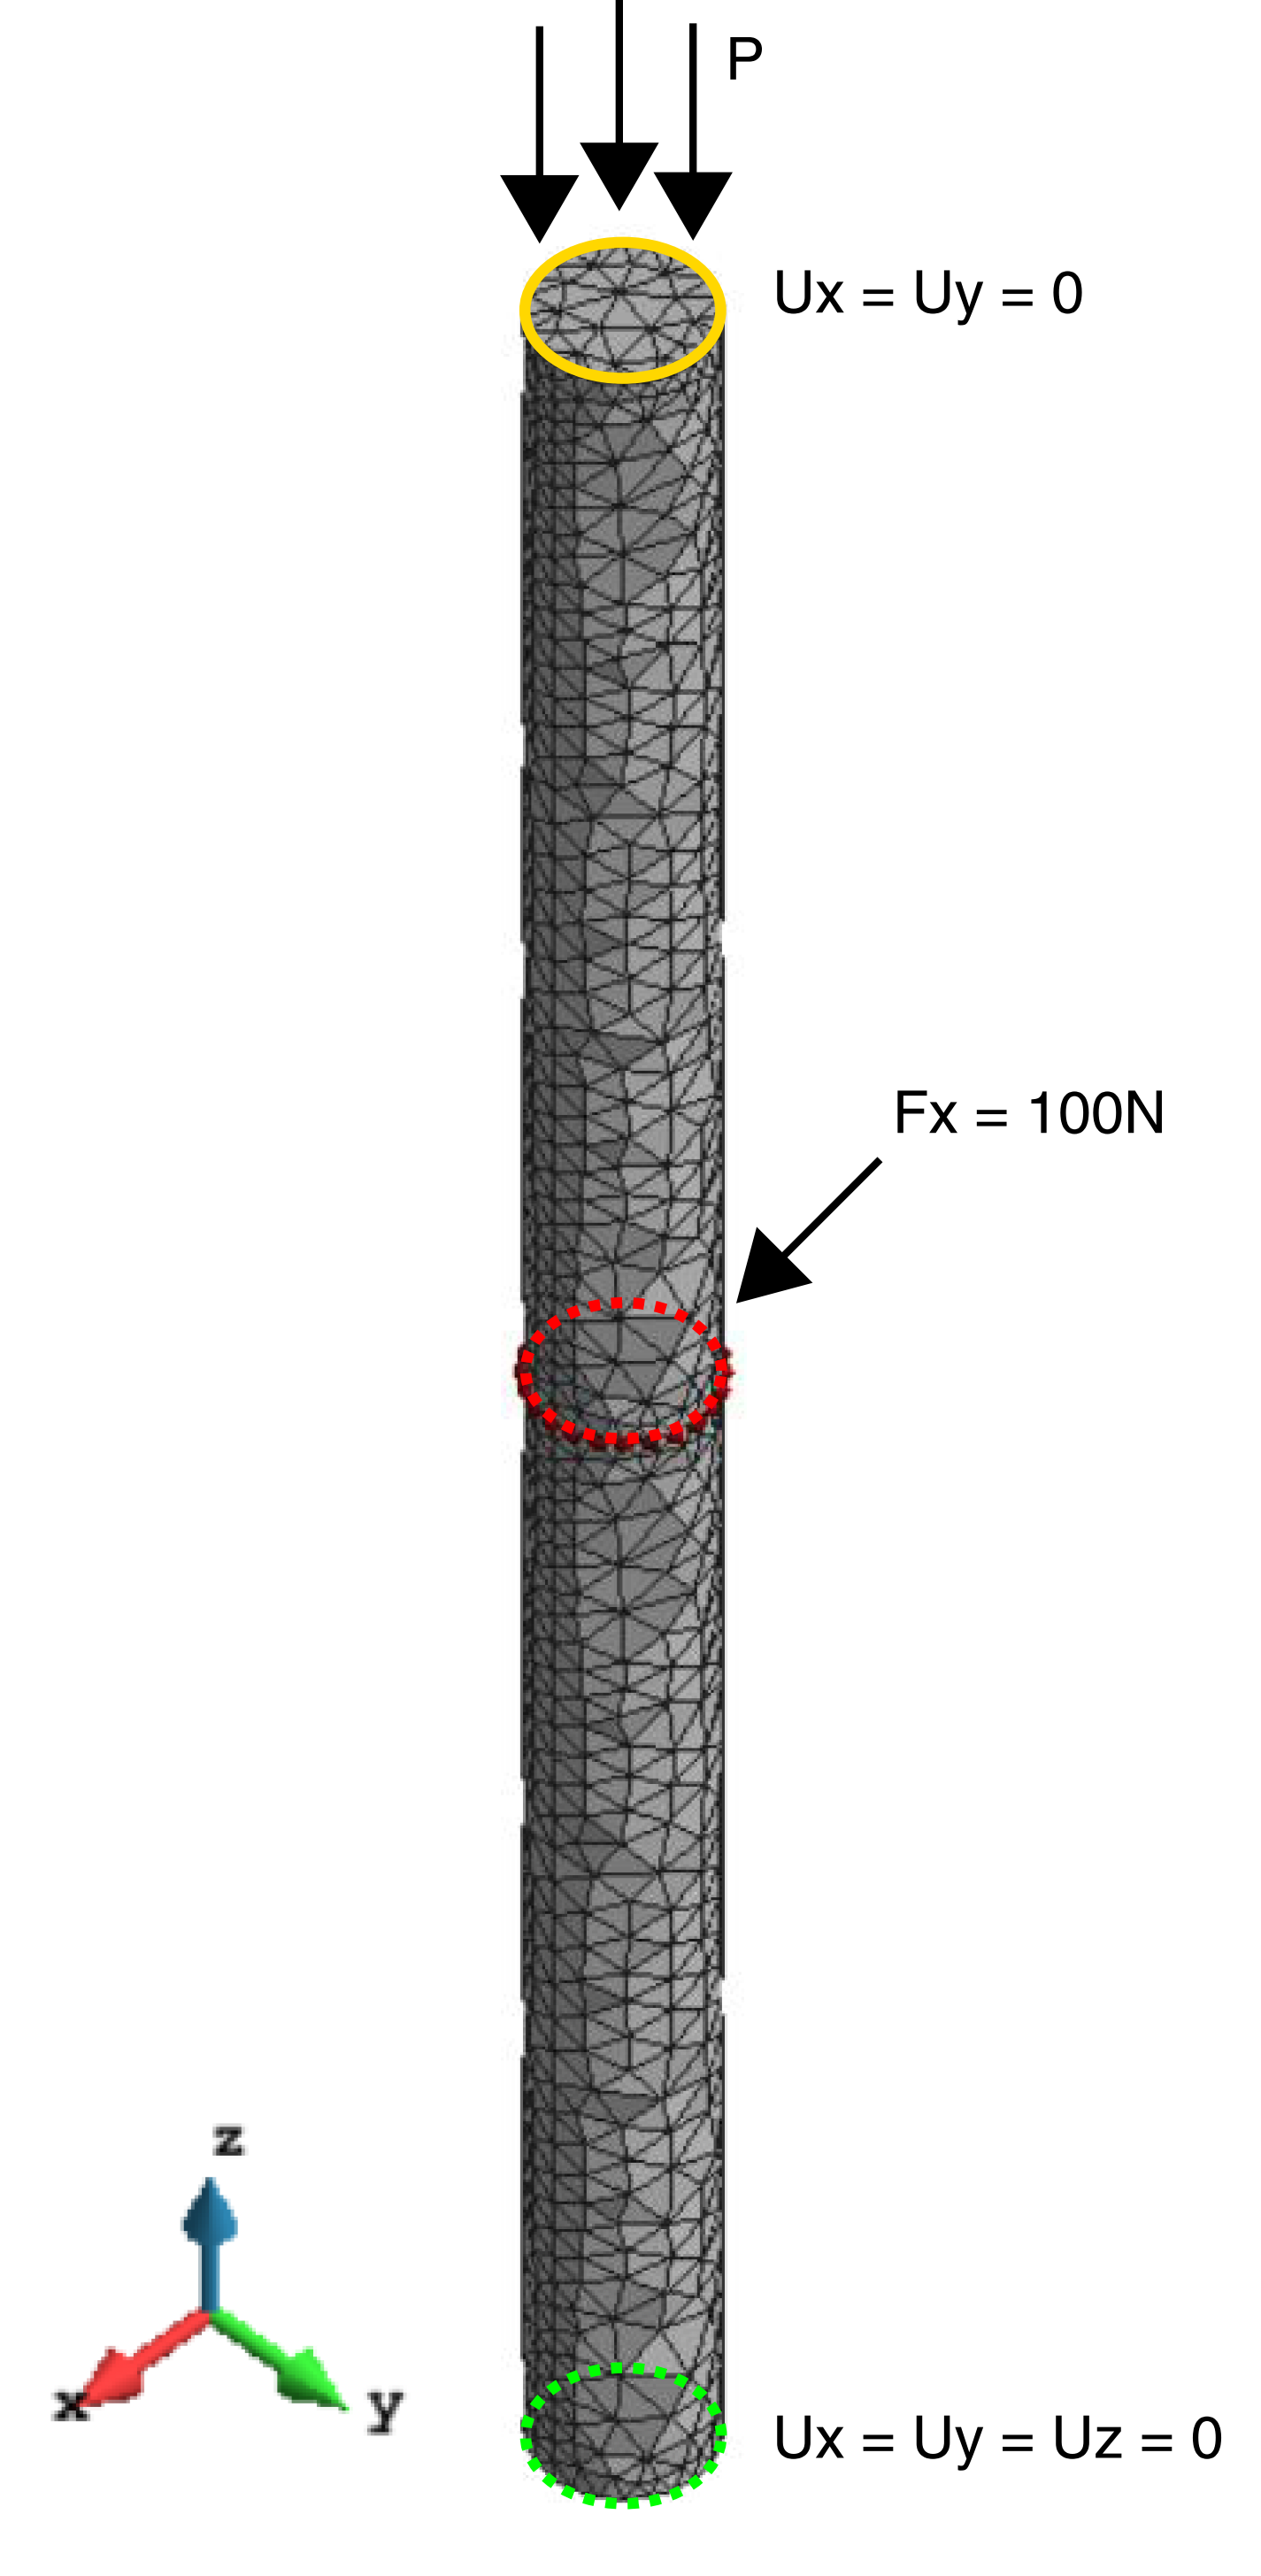
\includegraphics[height=12cm]{images/chs_buckling_setup}
	\caption{CHS buckling setup}
	\label{fig:chsbucklingsetup}
\end{figure}

A full derivation of the Euler case 4 buckling load using beam theory is presented in Appendix \ref{app:Derivation of Euler buckling load} in which the critical load corresponding to the first eigenvalue is:

\begin{equation} 
P_{crit} = \frac{4\pi^2 EI}{L^2} = 13, 222 kN
\label{eqchs_1}
\end{equation}

Due to the unpredictable nature of solving bifurcation problems with FEM a small side load $F_x = 0.1 kN$ is added to a horizontal ring of nodes at the beam's mid-span to encourage switching to the secondary equilibrium path defined by buckling in the XZ plane. Without this side load, or some other reliable source of imperfection, it is possible that the FE model would continue along the primary equilibrium path after the first critical point, instead of switching to a secondary path of buckling. Although the unstructured meshes used may provide enough asymmetry to act as a buckling catalyst, the severity of the imbalance would no doubt change from triangular to quadrilateral unstructured meshes, which may affect the results. Conversely, it's supposed that the applied small lateral load provides a consistent source of imperfection  of greater magnitude than the underlying mesh imbalances, thereby allowing an apples to apples comparison between triangular and quadrilateral meshes.

The first set of results for the analysis highlighting axial displacement (of the top end) vs axial load $P$ is presented below, with circles indicating the onset of instability. Post-critical behaviour has been omitted for clarity.

\begin{figure}[H]
	\centering
	\def\svgwidth{\columnwidth}
	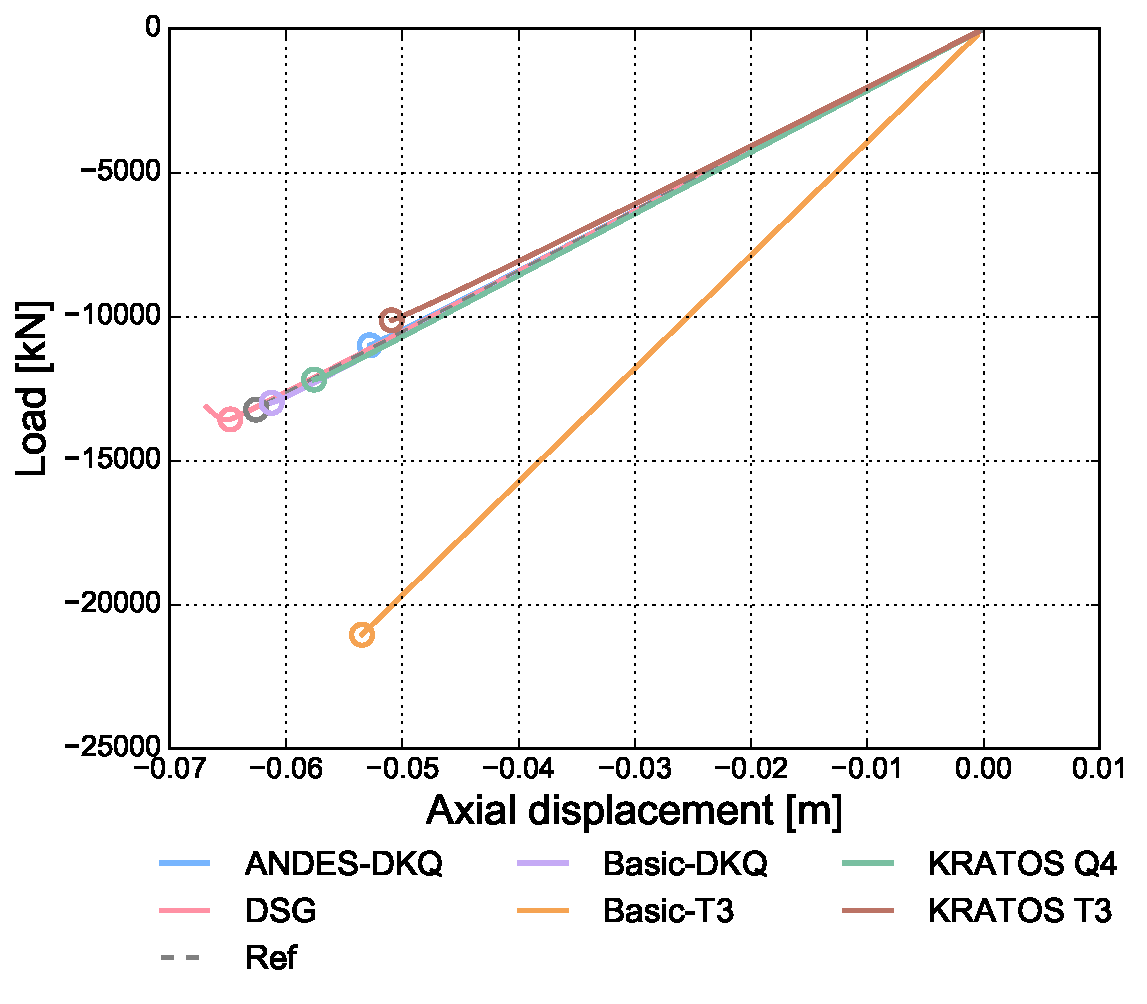
\includegraphics[width=12cm]{images/stability_chs_axial_disp.pdf}
	\caption{CHS buckling: axial displacement vs axial load}
	\label{pic:eulerchs1}
\end{figure}

The results above highlight the poor performance of the un-enhanced Basic-T3 element, with it's large over-estimation of the critical load a symptom of severe transverse shear locking. Accordingly, this poor performance also demonstrates the efficacy of the DSG element enhancements with the DSG results aligning quite well with the remaining elements and the reference beam theory solution (which has a first order displacement calculated from an axial stiffness of $EA/L$). The Basic-DKQ element is also quite close to the reference solution most likely because transverse shear locking is mitigated by the DKQ bending formulation while the effect of membrane locking (which this element is susceptible to) is minimized by the fine mesh employed (due to reduced element out of plane warping). Despite this, differences do indeed appear between the Basic-DKQ and ANDES-DKQ elements, the latter of which suggests a lower buckling limit along with the Kratos-T3 thin shell element. To gain more insight into this difference between these two elements and the rest, the axial load is plot against the lateral X-displacement taken at the beam mid-point $(x,y,z) = (D/2,0,L/2)$.

\begin{figure}[H]
	\centering
	\def\svgwidth{\columnwidth}
	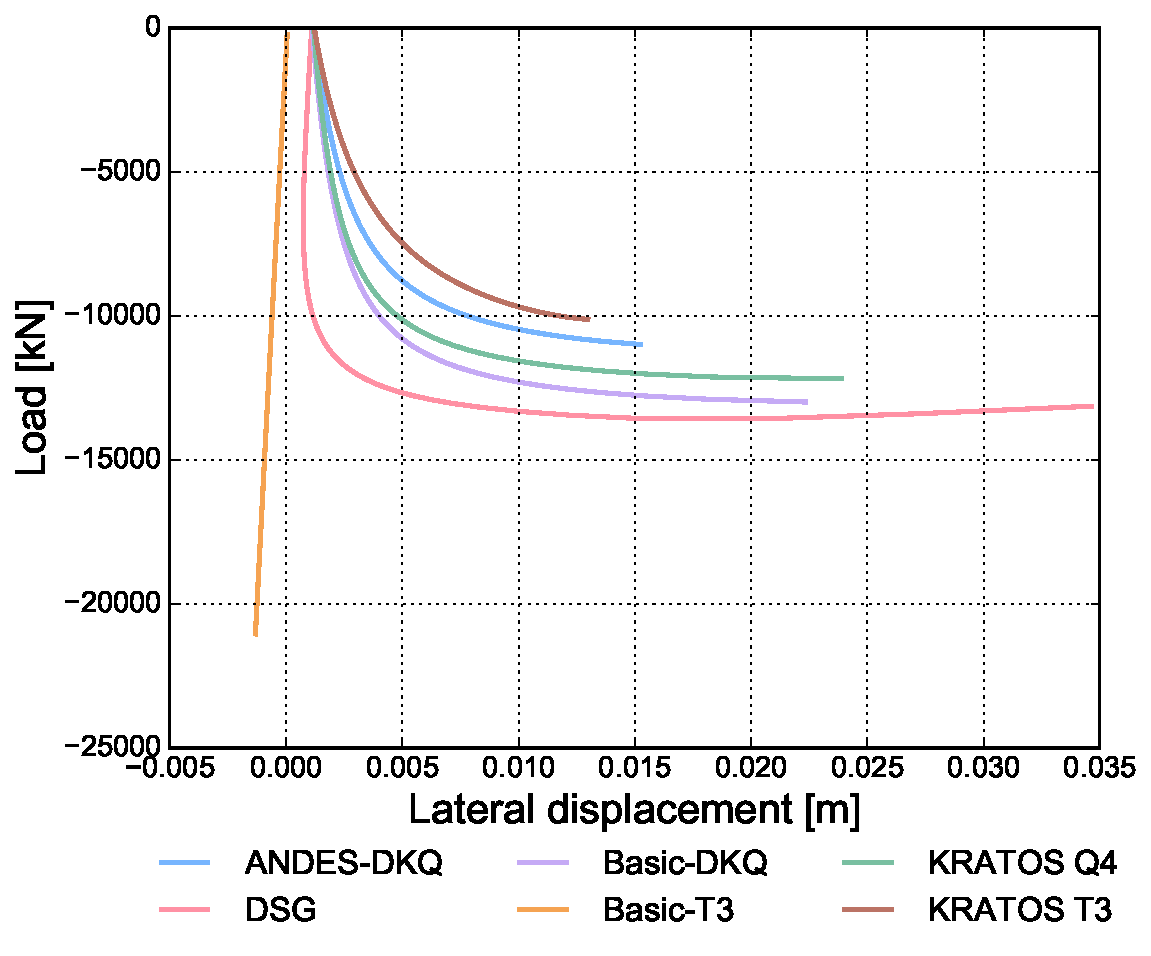
\includegraphics[width=12cm]{images/stability_chs_trans_disp.pdf}
	\caption{CHS buckling: lateral displacement vs axial load}
	\label{pic:eulerchs2}
\end{figure}

The alternative perspective presented above confirms the exceedingly poor performance of the Basic-T3 element once again. As previously identified, the ANDES-DKQ and Kratos-T3 elements predict low buckling loads for the system, however the plot above indicates that these are attached to reduced lateral displacements too (compared to the Kratos-Q4, Basic-DKQ and DSG elements). Clearly the various reasonable elements are expressing the system behaviour in different ways with the greatest difference occurring between the Kratos-T3 and DSG elements. To gain further insight into the behaviour of these two envelope cases, the following figures show X and Y displacements of the Kratos-T3 and DSG models at the onset of instability plot at 6.7x deformation with the same contour limits.

\begin{figure}[H]
	%\centering
	\subfloat[Kratos-T3 X-displacement]
	{\label{ref_label1}
		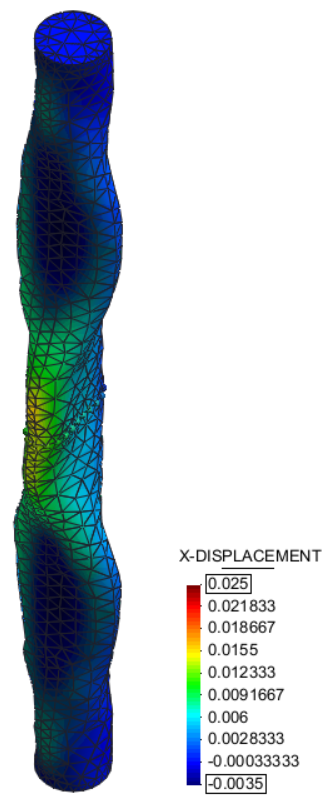
\includegraphics[width=3.5cm]
		{images/chs_kratos_tri_x.png}}
	\subfloat[DSG X-displacement]
	{\label{ref_label1}
		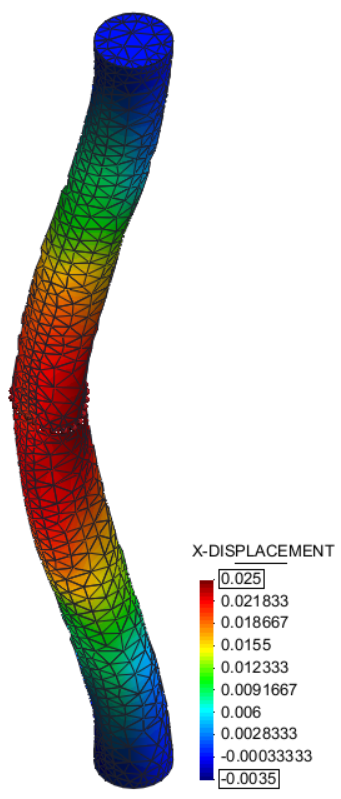
\includegraphics[width=3.5cm]
		{images/chs_dsg_x.png}}
	\subfloat[Kratos-T3 Y-displacement]
	{\label{ref_label2}
		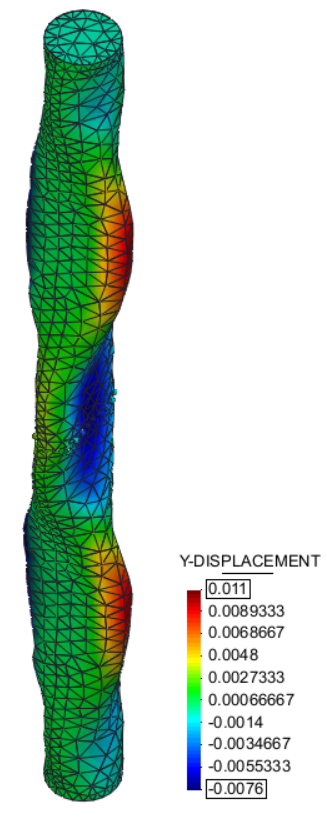
\includegraphics[width=3.5cm]
		{images/chs_kratos_tri_y.png}}
	\subfloat[DSG Y-displacement]
	{\label{ref_label2}
		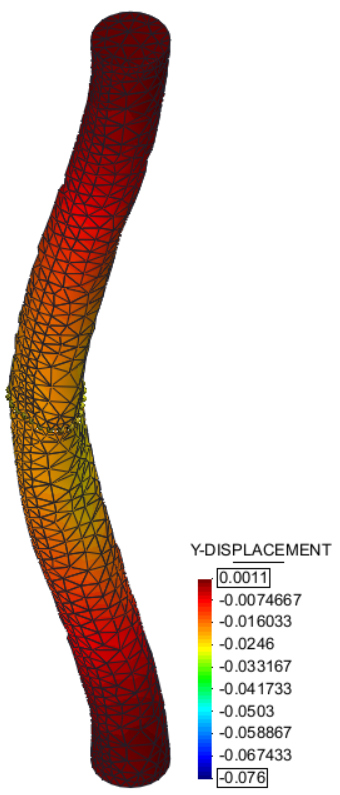
\includegraphics[width=3.5cm]
		{images/chs_dsg_y.png}}
	\caption{\label{chs buckling pics1}CHS buckling: Kratos-T3 and DSG displacement plots at the onset of instability}
\end{figure}

The plots above demonstrate the strikingly different structural behaviours modelled by the two elements using exactly the mesh, boundary conditions and loading conditions. Local ovalisation of the CHS appears to drive buckling in the Kratos-T3 case, whereas the DSG element predominantly maintains the circular cross section throughout and exhibits deformation one would expect from a beam element, explaining the close similarity between the DSG and reference beam results. The differences between the Kratos-T3 (3-parameter) and DSG (5-parameter) elements can be explained by their underlying formulation and the resolving power each posseses. Despite the slenderness ratio $R/t = 20$ of the problem being suitable for both thin and thick shell use, it's intuitive that at this point the 5-parameter model would be more reluctant than the 3-parameter model to predict out of plane bending behaviour, leading to ovalisation. Furthermore, the DSG element is computed with a single Gauss Point while the Kratos-T3 element is computed with 3 Gauss Points which confers a relative advantage in resolving complex local displacement fields (such as local ovalisation).

For completeness, the X and Y displacements of the ANDES-DKQ and Basic-DKQ models at the onset of instability are also plotted below with 6.7x deformation and equilibrated contour limits.

\begin{figure}[H]
	%\centering
	\subfloat[ANDES-DKQ X-displacement]
	{\label{ref_label1}
		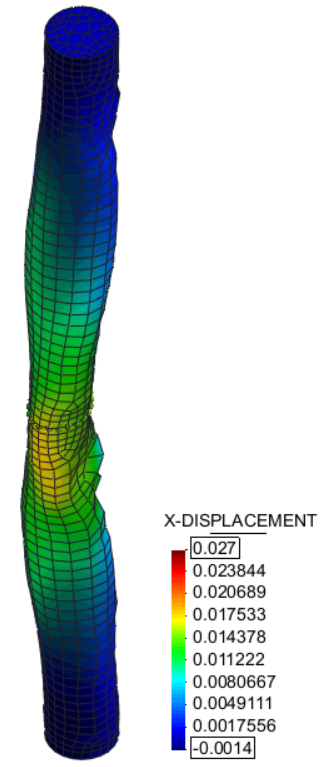
\includegraphics[width=3.5cm]
		{images/chs_thin_quad_x.png}}
	\subfloat[Basic-DKQ X-displacement]
	{\label{ref_label1}
		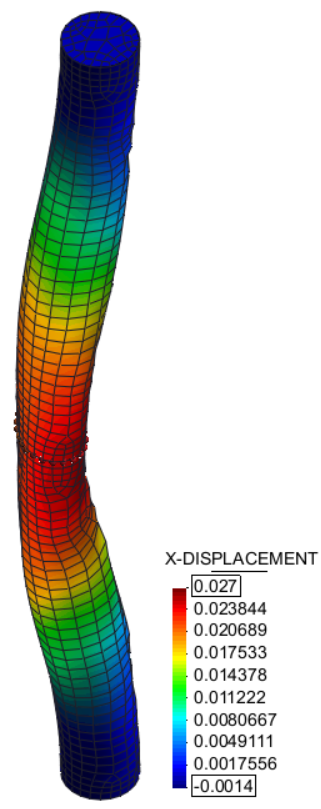
\includegraphics[width=3.5cm]
		{images/chs_thin_quad_basic_x.png}}
	\subfloat[ANDES-DKQ Y-displacement]
{\label{ref_label1}
	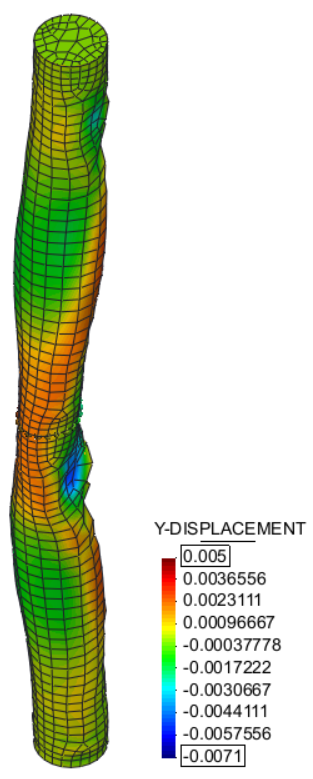
\includegraphics[width=3.5cm]
	{images/chs_thin_quad_y.png}}
\subfloat[Basic-DKQ Y-displacement]
{\label{ref_label1}
	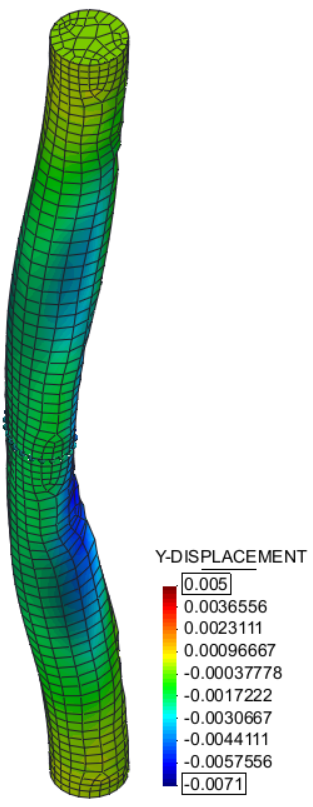
\includegraphics[width=3.5cm]
	{images/chs_thin_quad_basic_y.png}}
	\caption{\label{chs buckling pics2}CHS buckling: ANDES-DKQ and Basic-DKQ displacement plots at the onset of instability}
\end{figure}

In this comparison, the differences in deformation behaviour is solely due to the ANDES enhancement that mitigates membrane locking. An unstructured quadrilateral mesh of a curved surface, such as above, is a quintessential situation for membrane locking to arise. It can be seen that the ANDES-DKQ case exhibits ovalisation of the cross section as expected by it's similarity to the aforementioned Kratos-T3 results. Contrasting this, the Basic-DKQ results display an incredibly minor amount of ovalisation, reduced from it's enhanced counterpart solely due to unmitigated membrane locking, with a more classical beam deflection shape maintaining a relatively constant cross section throughout. Although the ANDES-DKQ and the Basic-DKQ have the same local displacement field resolving power of 4 Gauss Points and also have 3-parameter based enhanced bending formulations, the membrane formulation leading to the prevention or inclusion of membrane locking is the decisive factor here and evidently has a significant impact on the results obtained.

Through the comparison of results obtained with various elements employing different element enhancements it is clear that structural modelling with shells, as discussed in section \ref{Structural modelling with shells}, requires careful consideration of simplifications and assumptions made. For the analysed problem of a CHS beam buckling dimensional reduction can be reasonably varied between a 1D and 2D approach, as explored. Undertaking a one dimensional beam approach may yield quick and acceptable 'ballpark' results, such as Euler's buckling formula, but it also immensely filters the space of possible mechanical expressions resolvable, such as local ovalisation which was seen to form an important driver in some of the results obtained. However, simply adopting a two dimensional shell approach to the problem did not homogenize all results, as was seen. Element base formulations, element enhancements, element order and mesh were all important factors strongly affecting results and correspond to questions that must be answered upon entering the shell regime. 

\section{Shear wrinkling of plate}

Although classic Euler buckling is perhaps the most apparent phenomena that comes to mind when considering beam structures, the previous example highlights that local buckling effects can come to dominate the overall structural behaviour. Progressing along this vein, another local instability phenomena that can occur with I-sectioned beams is web buckling wherein the web manifests out of plane bubble-like deformation patterns.

The effect of element selection and enhancement on this phenomena can be considered by analysing a flat plate of $1.2m$ x $0.3m$ x $0.005m$ thick fully clamped on it's lower edge and laterally displaced by $U_x = \delta = 0.015m$ along it's top edge, roughly corresponding to an I-beam thin web under shear action. Material properties are taken as $E = 206.9 GPa$ and $\nu = 0.0$. The system setup is illustrated below:

\begin{figure}[H]
	\centering
	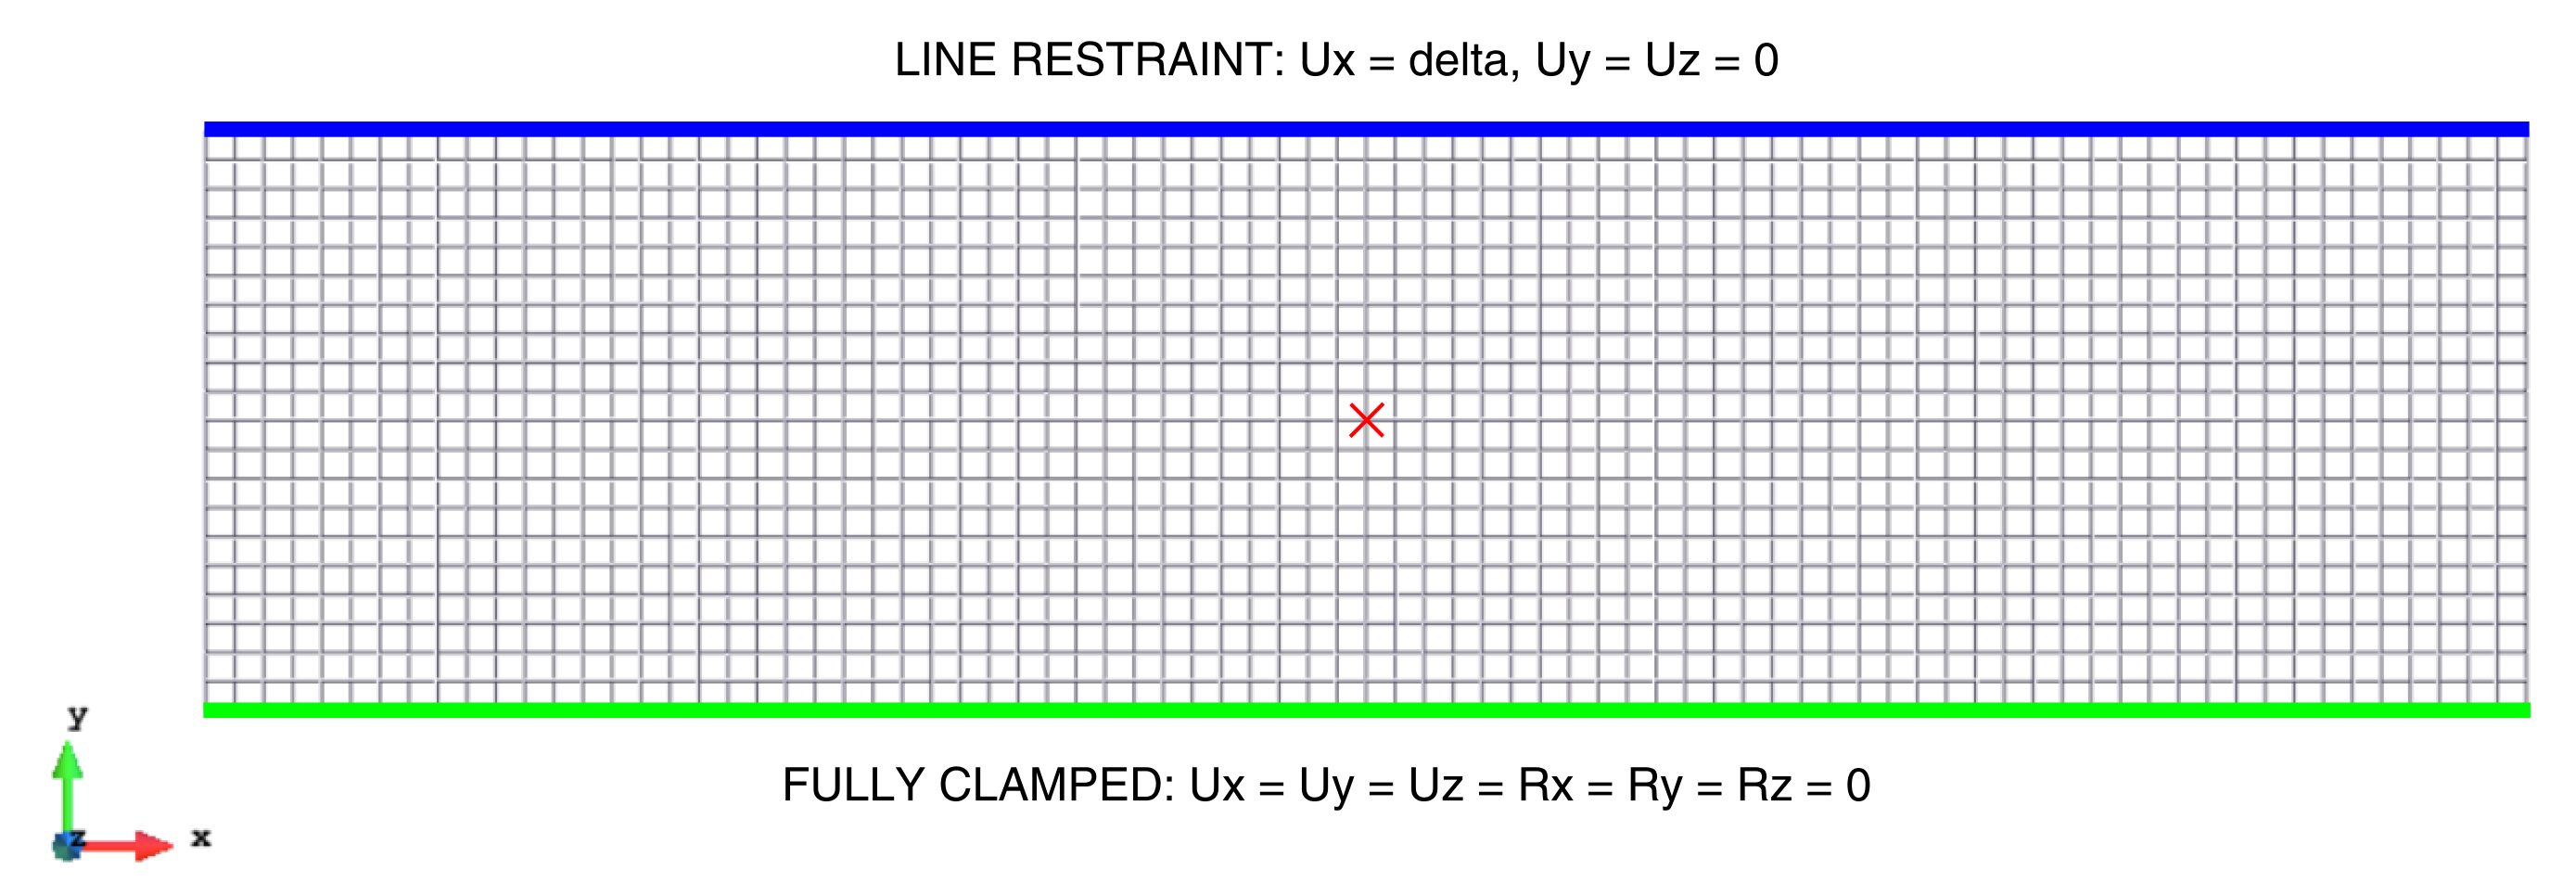
\includegraphics[width=12cm]{images/wrinkle_setup}
	\caption{Shear wrinkling of plate setup}
	\label{fig:wrinklesetup}
\end{figure}

As per the previous problem, bifurcation is encouraged with minor out of plane loading, this case being $F_z = -100N$ applied at the centre of the plate denoted by the red cross above. 

The first result presented is the imposed lateral displacement $\delta$ vs the lateral load, determined as the sum of all nodal lateral reactions $R_x$ along the displaced top edge.

\begin{figure}[H]
	\centering
	\def\svgwidth{\columnwidth}
	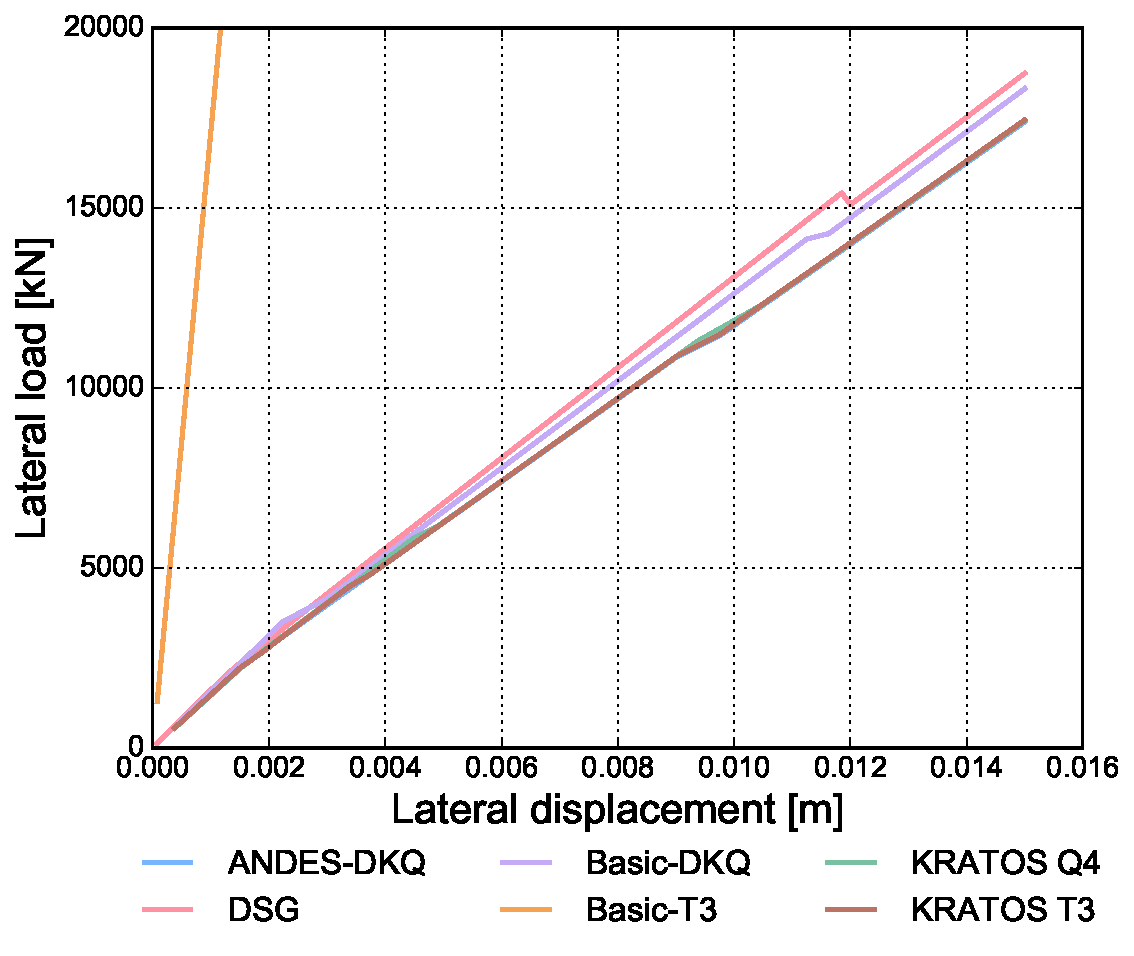
\includegraphics[width=12cm]{images/stability_wrinkle_axial_disp.pdf}
	\caption{Plate shear stability analysis: lateral displacement vs lateral load}
	\label{pic:wrinkle1}
\end{figure}

Separated from the other elements, the Basic-T3 element demonstrates spurious behaviour indicative of severe shear locking yet again. This also illustrates the effectiveness of DSG enhancements to inoculate against this deleterious phenomena. Apart from the Basic-T3 element, all remaining elements are grouped relatively close together exhibiting largely linear, albeit slightly softening, behaviour with apparent disturbances at lateral loads of roughly $4000N$ and $15000N$

To avail further insight of the problem, the out of plane displacement of the mid-point (denoted with a red cross in figure \ref{fig:wrinklesetup}) is plotted against the lateral load.

\begin{figure}[H]
	\centering
	\def\svgwidth{\columnwidth}
	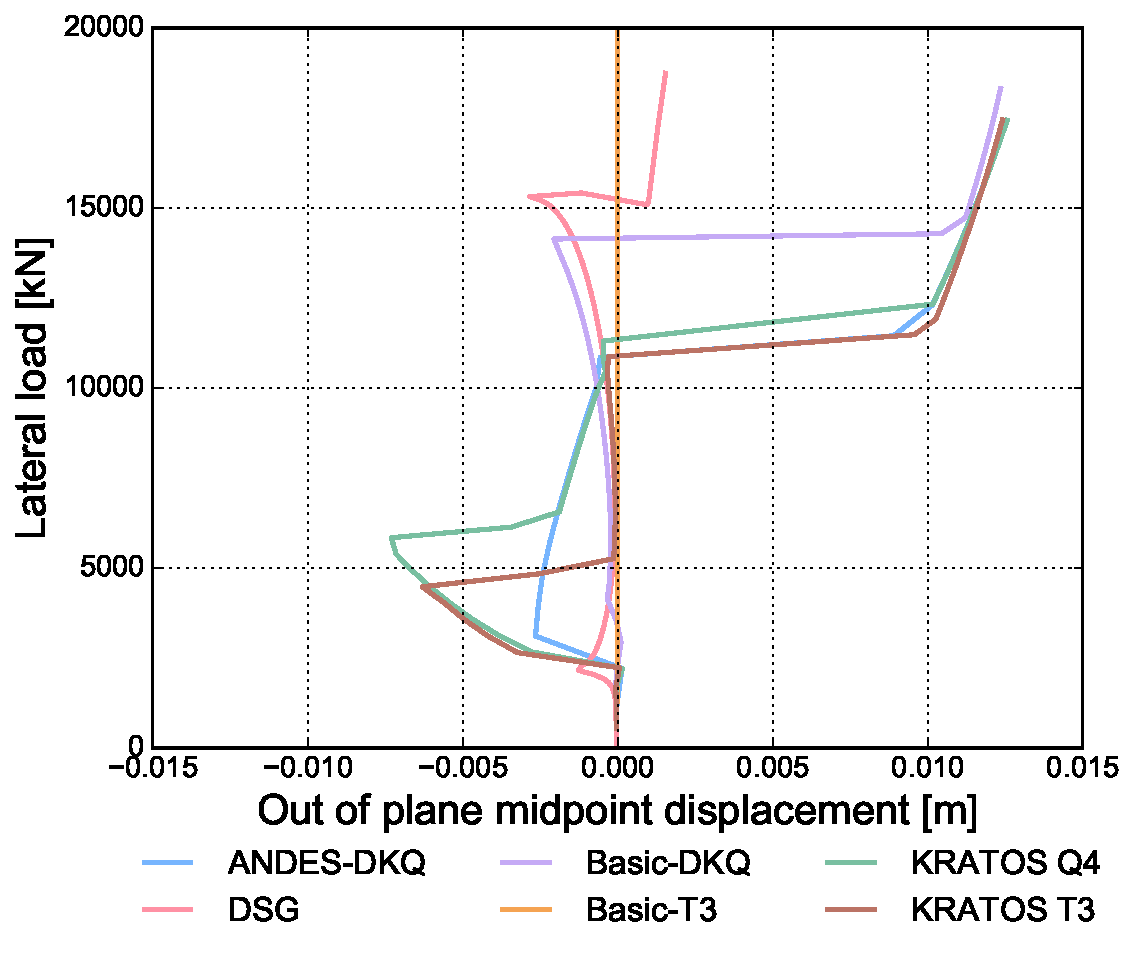
\includegraphics[width=12cm]{images/stability_wrinkle_pointtrans_disp.pdf}
	\caption{Plate shear stability analysis: out of plane mid-point displacement vs lateral load}
	\label{pic:wrinkle2}
\end{figure}

This perspective shift affords new clarity illustrating the Basic-T3 element never buckles during the whole analysis thereby explaining it's equilibrium path in figure \ref{pic:wrinkle1}. The remaining elements exhibit highly complex non-linear behaviour bifurcating between 3 (DSG) and 5 (Kratos-Q4 and Kratos-T3) times. Despite this, all reasonable elements demonstrate temporary stability in two zones: the secondary branch swaying leftwards in the load range of $(2500 - 6000)N$; and the final branch in the load range of $12000 N$ onwards. Despite this rough reconciliation, significant differences of structural behaviour still exist between the elements, which can be explored by examining the displacement contours at key points of interest.

In order to establish a general appreciation of the structural behaviour throughout the lateral reaction load range considered Z-displacement plots of the ANDES-DKQ element, fairly representative of the other elements' behaviour, at various key points on it's equilibrium path are presented below:

\begin{figure}[H]
	%\centering
		\subfloat[Response diagram]
	{\label{ref_label1}
		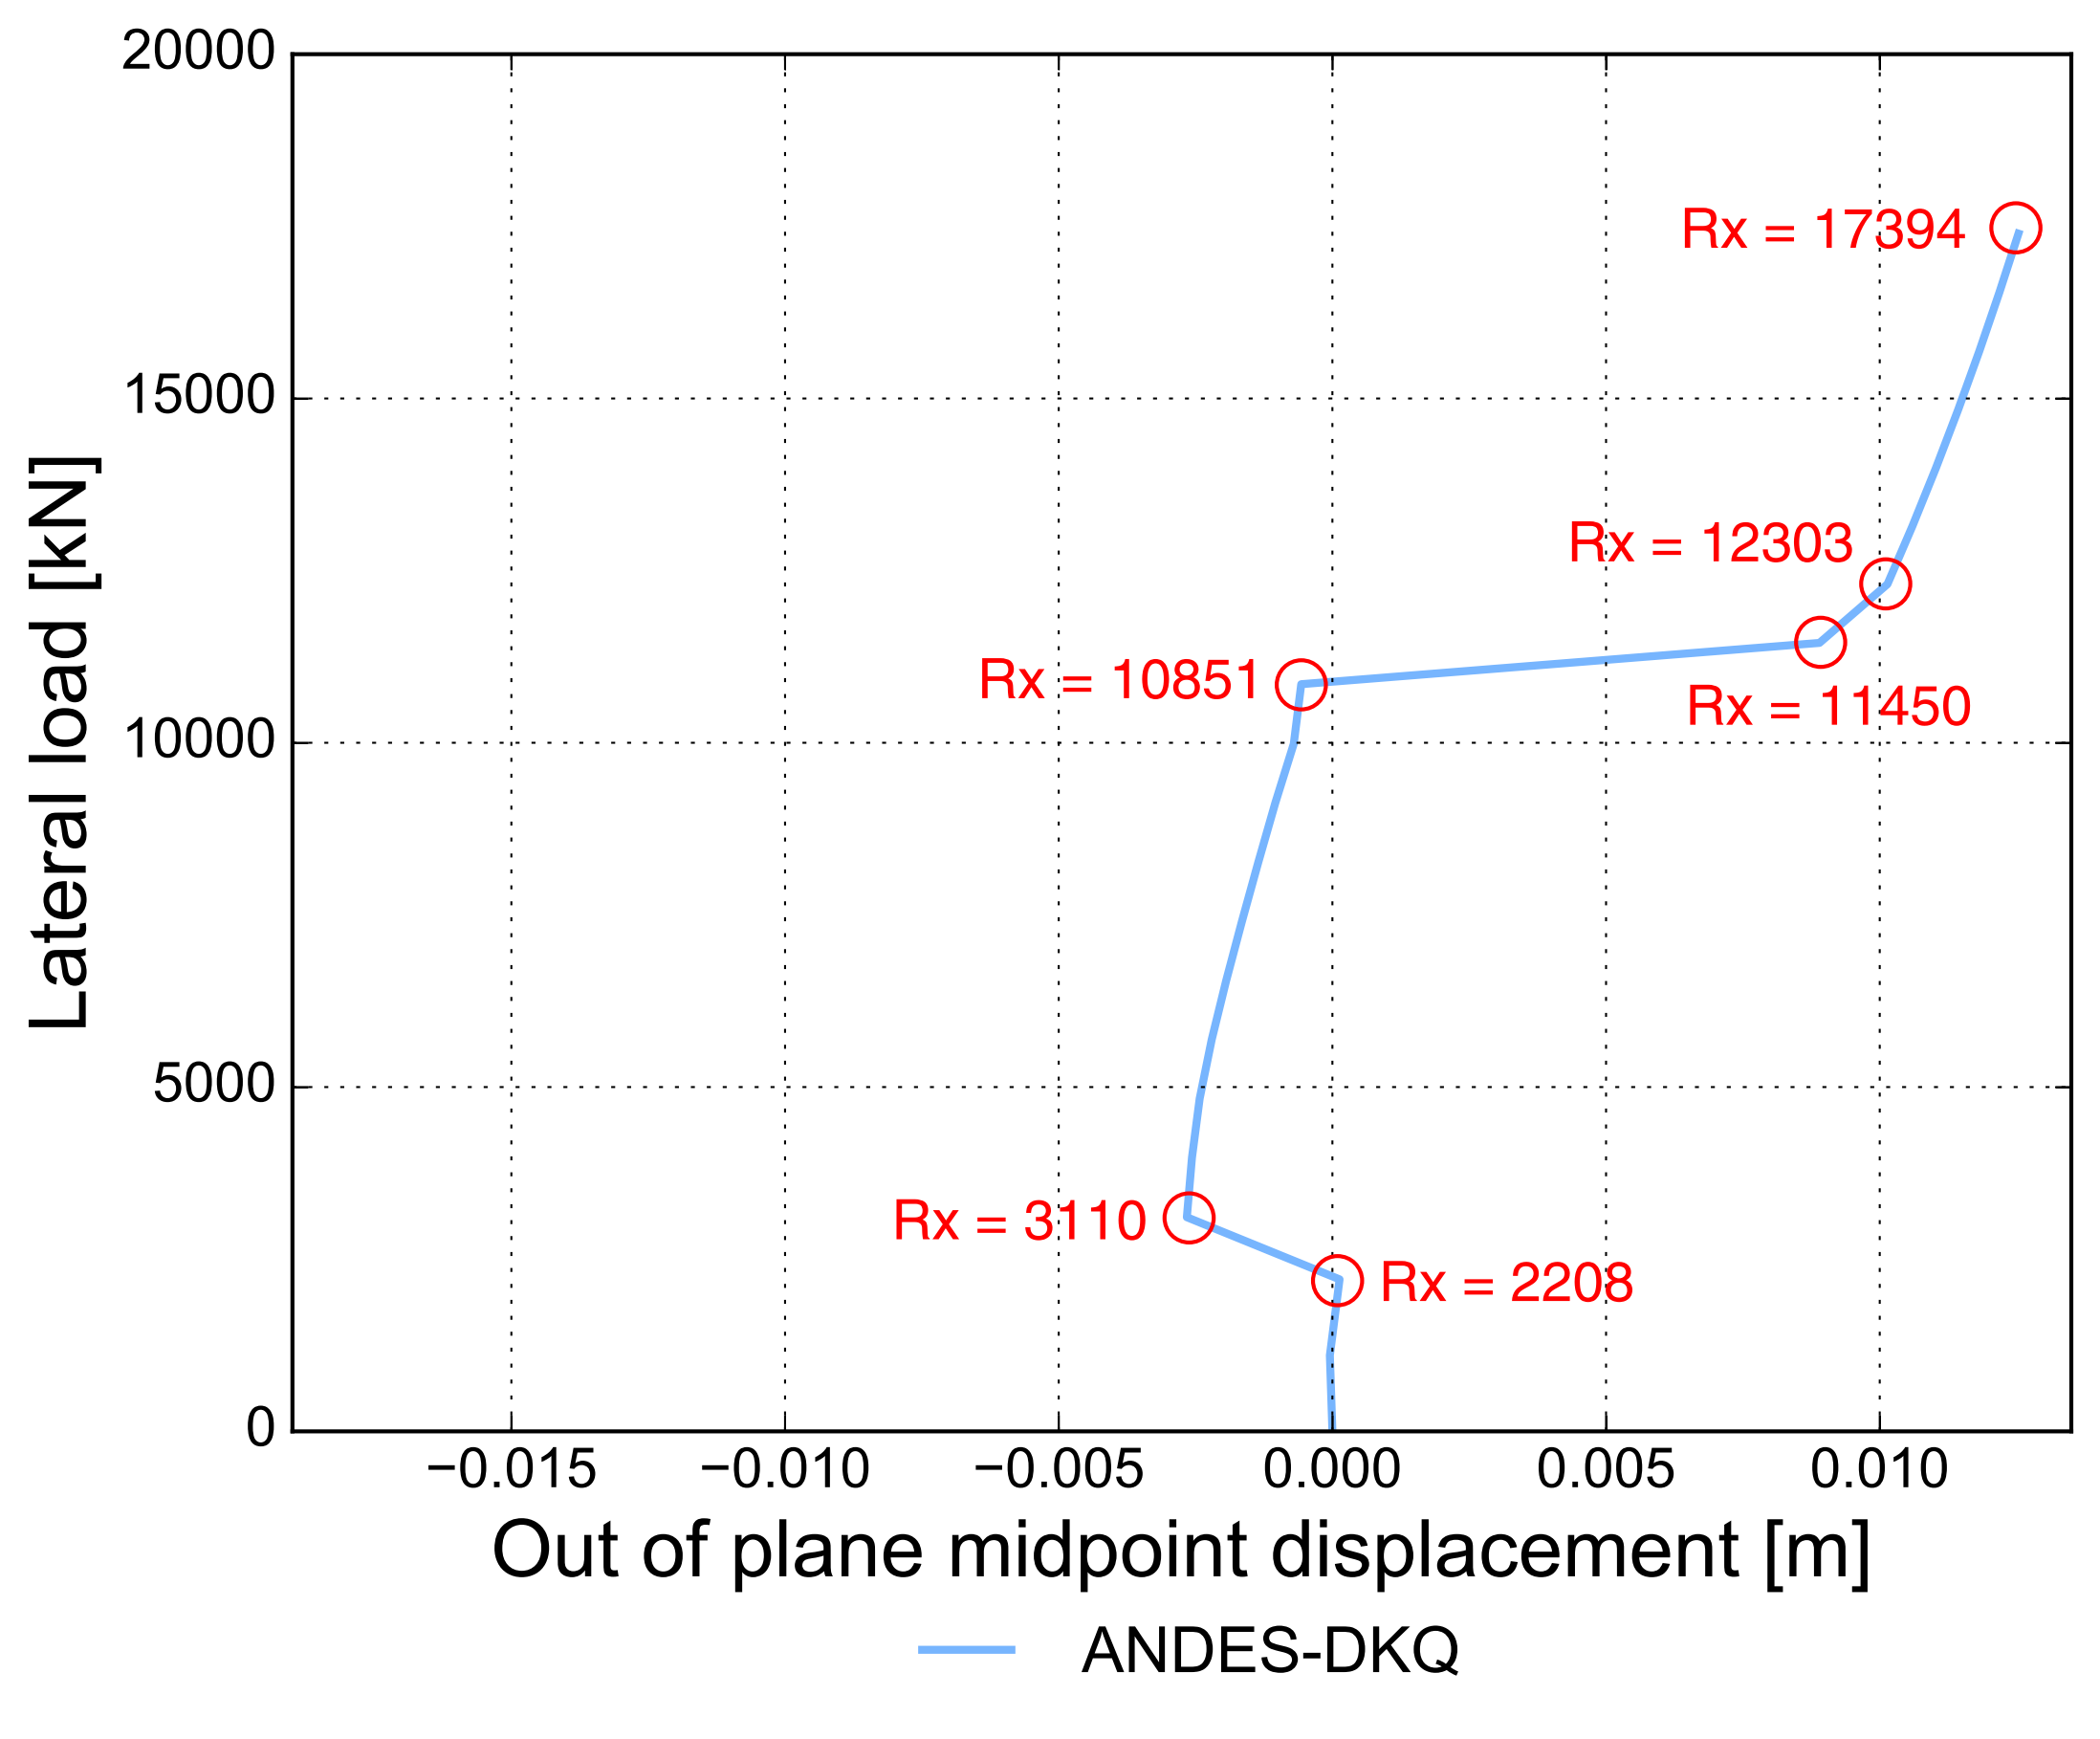
\includegraphics[width=10.0cm]
		{images/wrinkle_andes_NLgraph.png}}
	\subfloat[Contour colour scale]
	{\label{ref_label1}
		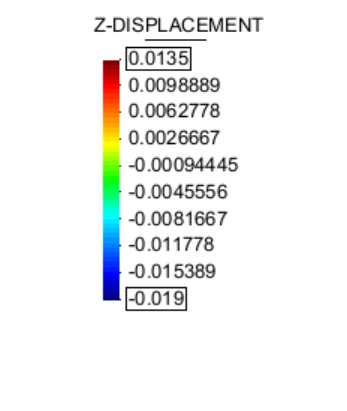
\includegraphics[width=4.0cm]
		{images/wrink_andes_scale.png}}
	\\
	\subfloat[Z-displacement @ Rx = 2208kN]
	{\label{ref_label1}
		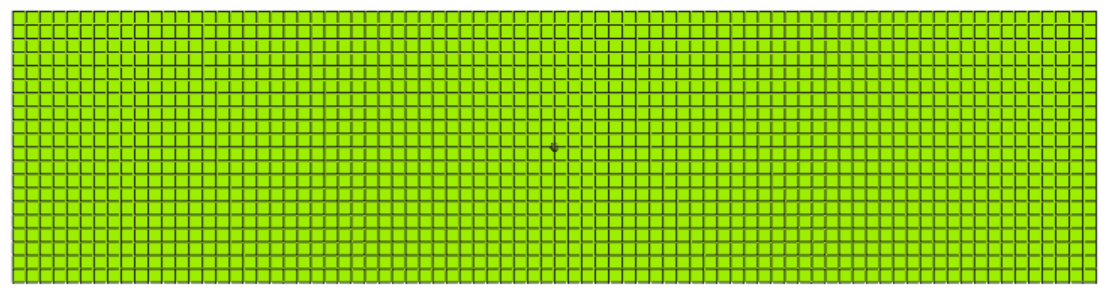
\includegraphics[width=7.0cm]
		{images/wrinkle_andes_t0_1.png}}
	\subfloat[Z-displacement @ Rx = 3110kN]
	{\label{ref_label1}
		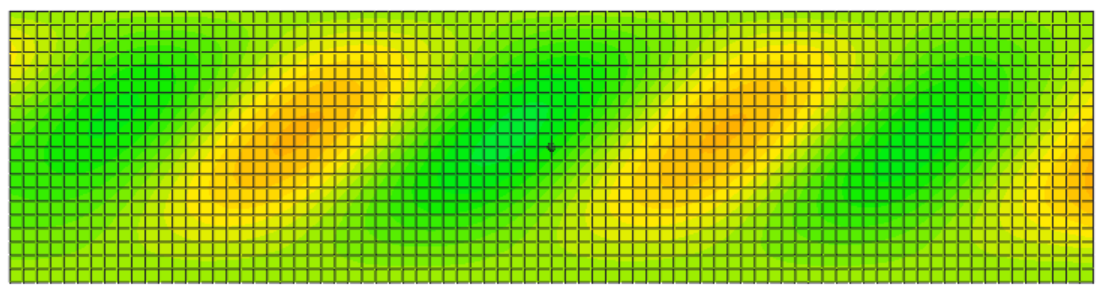
\includegraphics[width=7.0cm]
		{images/wrinkle_andes_t0_15.png}}
	\\
\subfloat[Z-displacement @ Rx = 10851kN]
{\label{ref_label1}
	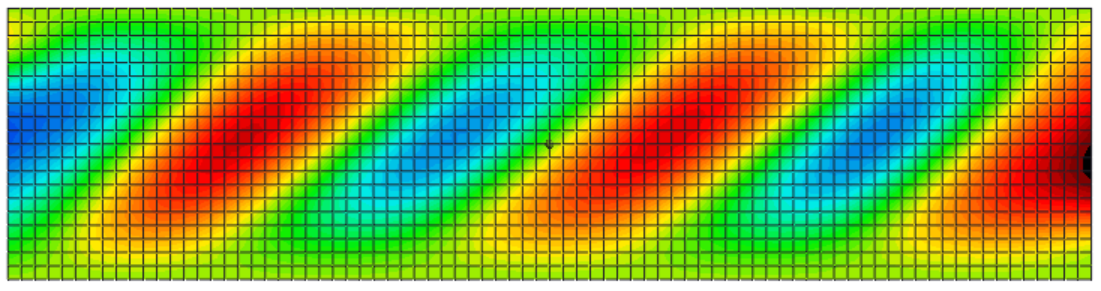
\includegraphics[width=7.0cm]
	{images/wrinkle_andes_t0_6.png}}
\subfloat[Z-displacement @ Rx = 11450kN]
{\label{ref_label1}
	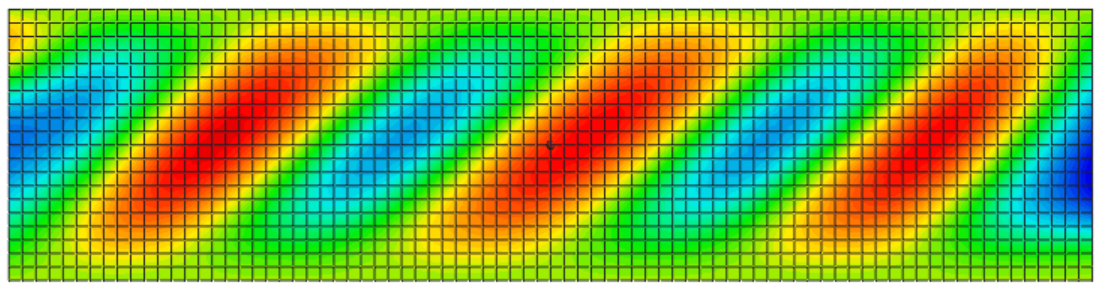
\includegraphics[width=7.0cm]
	{images/wrinkle_andes_t0_65.png}}
	\\
\subfloat[Z-displacement @ Rx =12303kN]
{\label{ref_label1}
	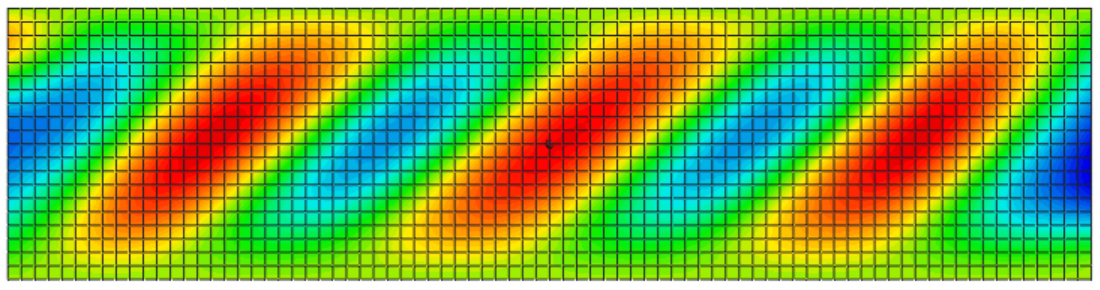
\includegraphics[width=7.0cm]
	{images/wrinkle_andes_t0_7.png}}
\subfloat[Z-displacement @ Rx = 17394kN]
{\label{ref_label1}
	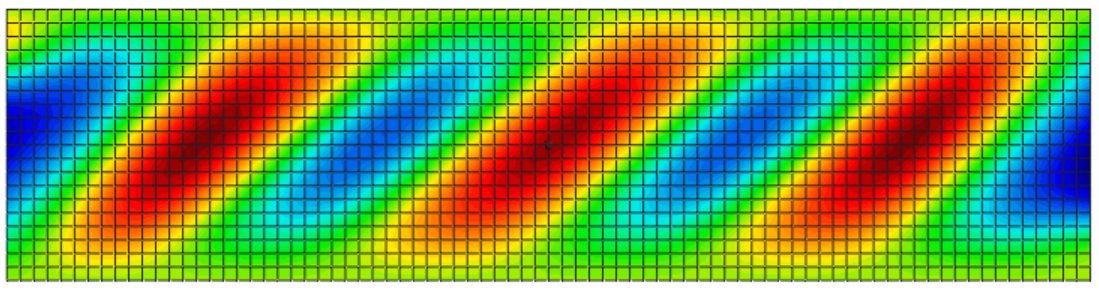
\includegraphics[width=7.0cm]
	{images/wrinkle_andes_t1_0.png}}
	\caption{\label{wrinkle 3}Plate wrinkling: ANDES-DKQ Z-displacement plots over equilibrium path}
\end{figure}

Plot (c) above shows the stressed unbuckled plate acting in pure membrane action with no developed out of plane displacement (other than that due to the minor point load) just before the onset of instability. Plot (d) highlights the deformation pattern in the secondary equilibrium path, which, for many of the other elements considered, constitutes the first zone of temporary stability as discussed before. A significant loss of membrane stiffness is somewhat tempered by the activation of the plate's bending stiffness via the relatively minor local curvature developed. Progressing to plot (e) illustrates the developing magnitude of the out of plane displacements and gradual re-distribution of the plate's buckling mode into a pattern of shorter period. The shift from state (e) to state (f) and finally to state (g) marks the transition to the final tightly defined buckling pattern of 3 peaks and 2 troughs, from an initial diffuse pattern of 2 peaks and 2 troughs, which activates more of the bending stiffness due to the higher curvatures involved. The final state (h) highlights the development and utilisation of this buckling mode which forms the second common zone of temporary stability among the other elements considered.

With a greater appreciation of the structural behaviour at hand, the different contours of the DSG and Kratos-T3 element, representing 5-parameter and 3-parameter based formulations respectively, are considered at the two zones of temporary stability.

\begin{figure}[H]
	%\centering
	\subfloat[Kratos-T3 @ $\delta = 0.0025m$]
	{\label{ref_label1}
		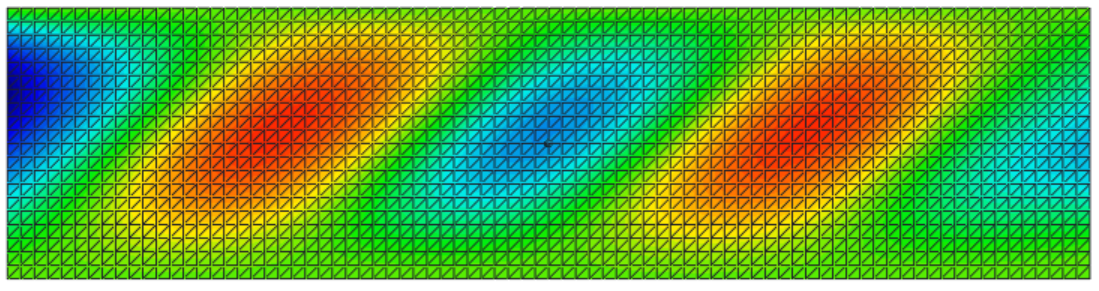
\includegraphics[width=6.25cm]
		{images/wrinkle_kratosT3_t0_15.png}}
	\subfloat[DSG @ $\delta = 0.0025m$]
	{\label{ref_label1}
		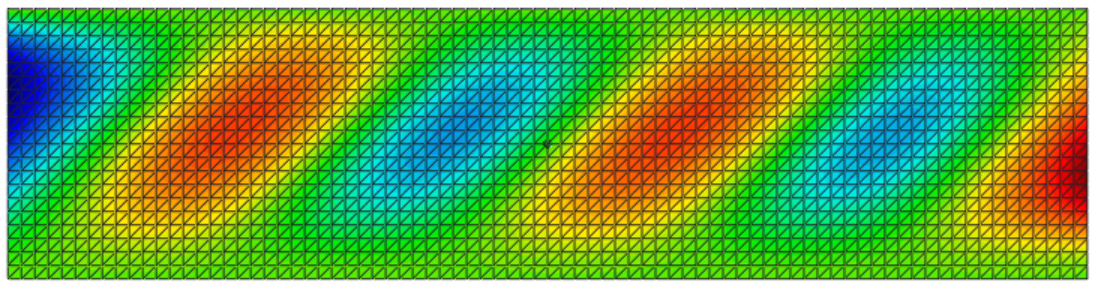
\includegraphics[width=6.25cm]
		{images/wrinkle_dsg_t0_15.png}}
	\subfloat[Legend]
	{\label{ref_label1}
		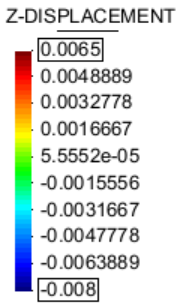
\includegraphics[width=1.5cm]
		{images/wrinkle_dsg_scale_t0_15.png}}
	\\
	\subfloat[Kratos-T3 @ $\delta = 0.015m$]
{\label{ref_label1}
	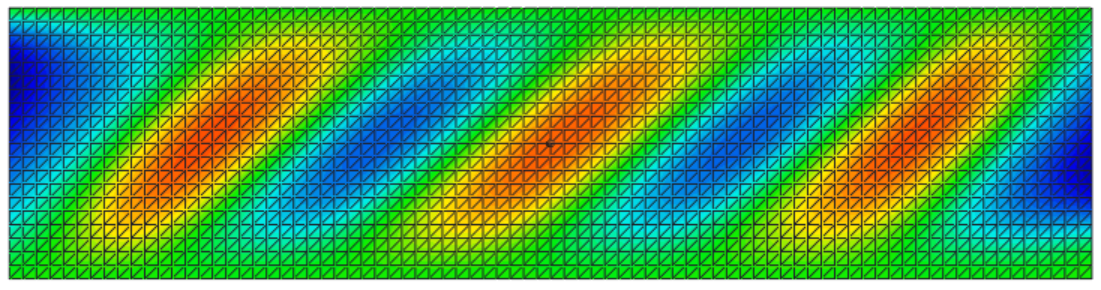
\includegraphics[width=6.25cm]
	{images/wrinkle_kratosT3_t1_0.png}}
\subfloat[DSG @ $\delta = 0.015m$]
{\label{ref_label1}
	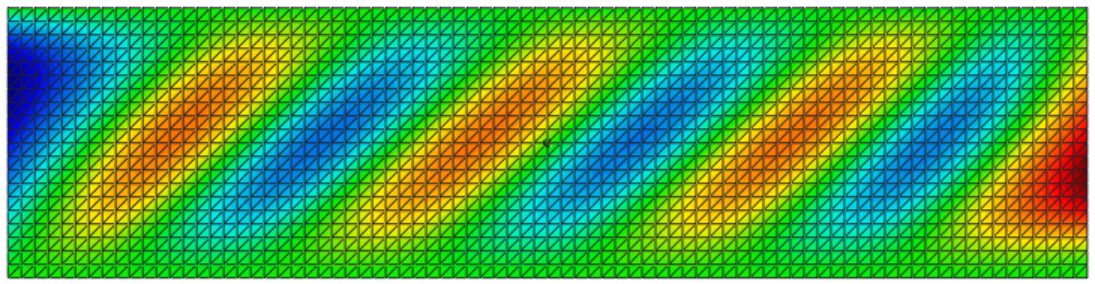
\includegraphics[width=6.25cm]
	{images/wrinkle_dsg_t1_0.png}}
\subfloat[Legend]
{\label{ref_label1}
	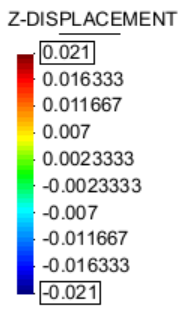
\includegraphics[width=1.5cm]
	{images/wrinkle_dsg_scale_t1_0.png}}
	\caption{\label{wrinkle 4}Plate wrinkling: Kratos-T3 and DSG Z-displacement plots over equilibrium path}
\end{figure}

Although the displacement contours above minimize the differences suggested by figure \ref{pic:wrinkle2} the DSG element displays a shorter buckling bubble period than the 3-parameter Kratos-T3 element. Intuitively, the phenomenological association between locking (which the DSG element largely mitigates, but remains in it's "genes" due to it's 5-parameter foundation) and greater stiffness can be superimposed on the general effect of higher stiffness's reducing oscillation periods in general physics, explaining to the reduced spacing between peaks (and troughs) in the DSG element. Despite this difference, it must be noted that compared to the Basic-T3 element the DSG element performs admirably given it's heritage. Furthermore, the smallest slenderness ratio of $L/t = 0.3/0.005 = 60$ places this analysis firmly in the realms of thin plates, rendering 5-parameter based elements as "fish out of water".

As per the above considerations, plots of the ANDES-DKQ and Basic-DKQ elements at the two temporary stability points are presented below:

\begin{figure}[H]
	%\centering
	\subfloat[ANDES-DKQ @ $\delta = 0.0025m$]
	{\label{ref_label1}
		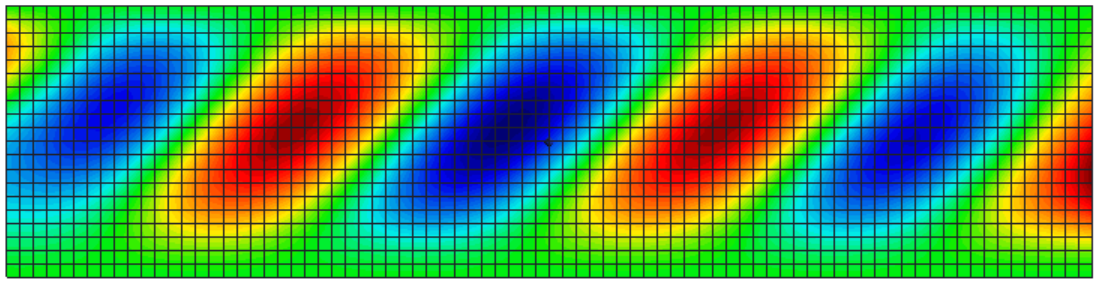
\includegraphics[width=6.25cm]
		{images/wrinkle_andes_comp_t0_15.png}}
	\subfloat[Basic-DKQ @ $\delta = 0.0025m$]
	{\label{ref_label1}
		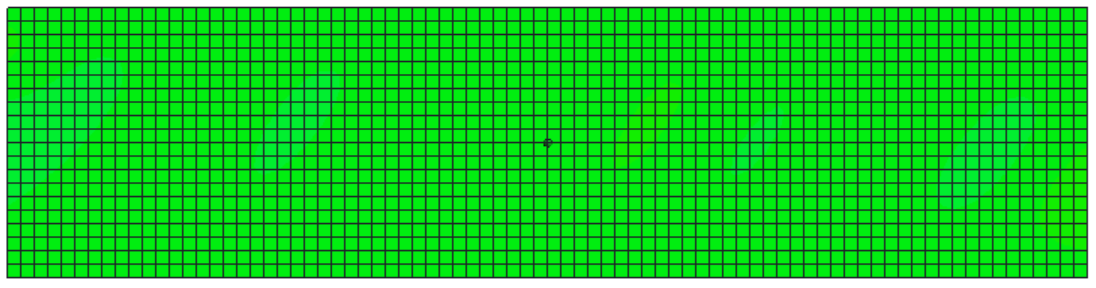
\includegraphics[width=6.25cm]
		{images/wrinkle_basic_andes_t0_15.png}}
	\subfloat[Legend]
	{\label{ref_label1}
		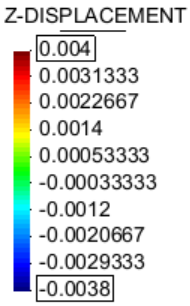
\includegraphics[width=1.5cm]
		{images/wrinkle_andes_comp_scale_t0_15.png}}
	\\
	\subfloat[ANDES-DKQ @ $\delta = 0.015m$]
	{\label{ref_label1}
		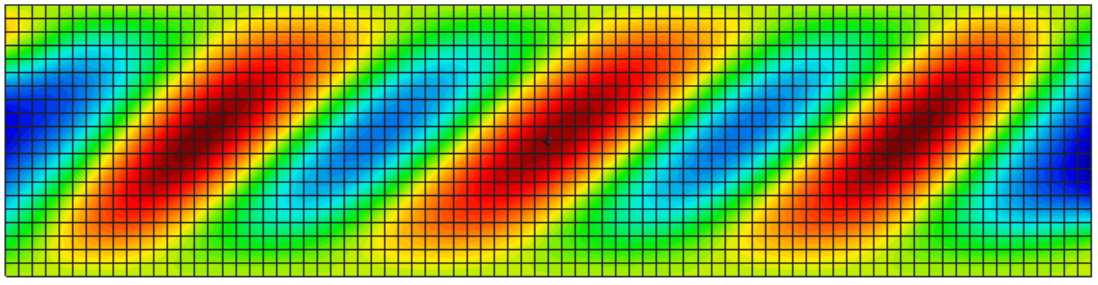
\includegraphics[width=6.25cm]
		{images/wrinkle_andes_comp_t1_0.png}}
	\subfloat[Basic-DKQ @ $\delta = 0.015m$]
	{\label{ref_label1}
		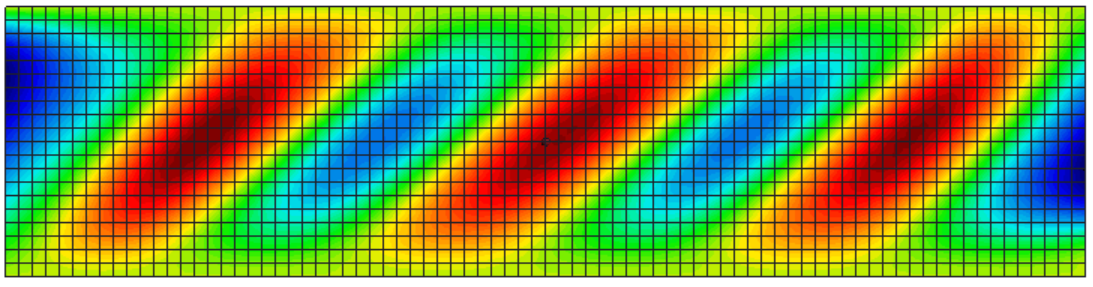
\includegraphics[width=6.25cm]
		{images/wrinkle_basic_andes_t1_0.png}}
	\subfloat[Legend]
	{\label{ref_label1}
		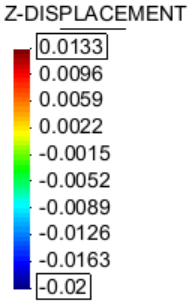
\includegraphics[width=1.5cm]
		{images/wrinkle_andes_comp_scale_t1_0.png}}
	\caption{\label{wrinkle 5}Plate wrinkling: ANDES-DKQ and Basic-DKQ Z-displacement plots over equilibrium path}
\end{figure}

Given that the problem considered is almost perfectly flat (except due to the destabilising central point load) and relatively free of membrane locking, one would expect no appreciable difference between these two elements (which only differ by the ANDES membrane enhancement), although the plots above suggest otherwise. The Basic membrane formulation clearly delays bifurcation into the secondary path that the ANDES formulation switches to at this load level, along with most other elements considered. Thus, it is likely that the Basic-DKQ element experienced very minor amounts of membrane locking depriving sufficient bending energy allocation and delaying the onset of autocatalytic out of plane displacements, themselves the precursor to entering the secondary branch. Despite this delayed onset of buckling, the final state of the system is demonstrably bending (and hence bending formulation) dominated, with both elements converging to near identical displacement patterns and magnitudes. Thus, in general, from this comparison, it seems apparent that membrane formulations regulate the onset of instability of the problem while bending formulations determine the buckled mode shapes.

The last perspective considered is the maximum (across the whole domain) absolute out of plane displacement against lateral load, which offers a simplified bulk characterisation of the structural behaviour.

\begin{figure}[H]
	\centering
	\def\svgwidth{\columnwidth}
	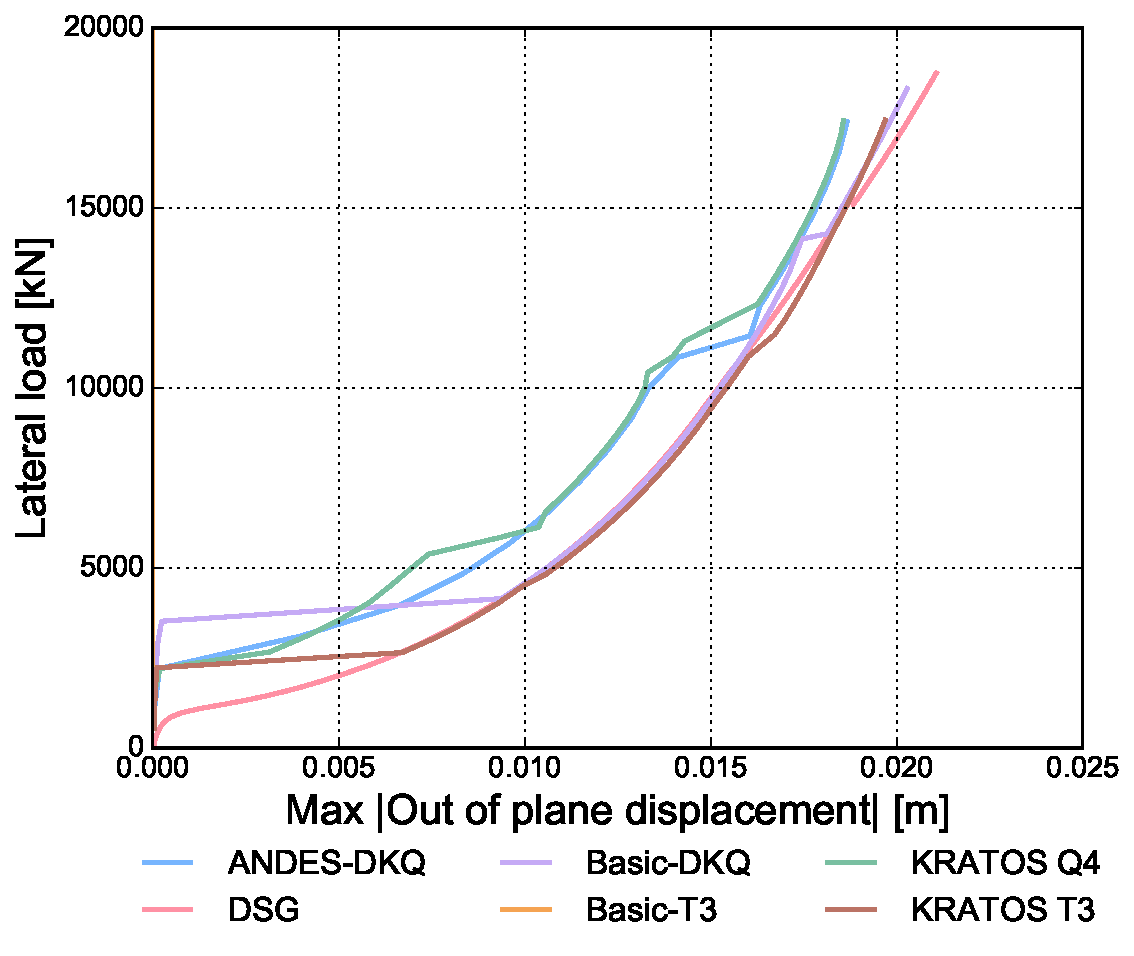
\includegraphics[width=12cm]{images/stability_wrinkle_abstrans_disp.pdf}
	\caption{Plate shear stability analysis: maximum absolute out of plane displacement vs lateral load}
	\label{pic:wrinkle3}
\end{figure}

The figure above summarises the bulk behaviour of the structural and highlights key phenomena of interest in a general sense. The initial vertical paths of the elements (the Basic-T3 path is entirely vertical) represent the deformation under pure membrane action which shortly after break laterally upon bifurcating into the secondary branch For instance, the late bifurcation of the Basic-DKQ element due to it's basic membrane formulation is clearly exposed. After bifurcating, as explored previously, the different elements enter into slightly different buckling modes, explaining the variation of paths between elements, however all buckling modes substitute the lost membrane stiffness with the activated bending stiffness leading to the shared hardening behaviour across all elements.

Complementing the summary of how element enhancements affect the CHS buckling analysis, the plate shear wrinkling also confirms the significant effect of element formulation and enhancement selection in the shell regime. Membrane technologies were found to be key in regulating the onset of buckling, with the un-enhanced membrane formulations either considerably delaying bifurcation (Basic-DKQ) or preventing it completely (Basic-T3). Some interplay with bending technologies is also present in determining initial bifurcation, explaining the difference between the Basic-T3 and DSG element behaviours, both of which have the same membrane formulation. The remaining enhanced membrane formulations of ANDES (ANDES-DKQ, Kratos-T3) and EAS (Kratos-Q4) predict similar points of buckling as per figure \ref{pic:wrinkle3}. This example highlights the importance of selecting appropriate element technologies not only based on the initial state of the system (which, in this case, a basic membrane formulation would suffice) but also on the predicted deformed state of the system (where a basic membrane formulation is insufficient).

 Upon bifurcation, the bending formulation and technologies largely determined the buckling shape exhibited by the system. The proper selection of a 3 or 5 parameter based formulation suitable to the problem considered appears to be of the utmost importance. Although the 5-parameter based DSG element achieved quite similar results to the 3-parameter based elements naturally suitable to slender problem, differences were nonetheless all too apparent, suggesting that element technologies themselves aren't the silver bullet to all problems, but are most effective when applied to base formulations inherently suitable to the problem considered.